\documentclass[../../main.tex]{subfiles}

\begin{document}

\subsection{Motivation}

It is considered a time series classification problem. This task is solved using ODE-RNN model. The ODE-RNN architecture was decribed in \cite{Samokhina}.

\subsection{Problem statement}

Given a multivariate time series:

$$\mathfrak{D} = \{(x_i, y_i)\}, \quad i = \overline{1, n}, \quad x_i \in \mathbb{R}^m.$$

\noindent
The problem of time series intervals classification is solved. We have to define if there is a P300 potential on the EEG interval.

Optimization task:

$$\hat{\theta} = \arg\max\limits_{\theta}L(\theta, \mathbf{X}).$$

\subsection{Problem solution}

ODE-LSTM is based on standard LSTM architecture but the continuity of hidden state is added. Hidden state of LSTM is a pair $(\mathbf{c}_t, \mathbf{h}_t)$, where $\mathbf{c}_t$ is a long term memory state, $\mathbf{h}_t$ is a hiden state. The function $f_\theta(\mathbf{x}_{t+1}, (\mathbf{c}_t, \mathbf{h}_t), \mathbf{1}) \rightarrow (\mathbf{c}_{t+1}, \mathbf{h}_{t+1})$ that updates these states can be described using the following equations:

$$\mathbf{z}_{t+1} = \tanh(\mathbf{W}_z\mathbf{x}_{t+1} + \mathbf{R}_z\mathbf{h}_t + \mathbf{b}_z)$$
$$\mathbf{i}_{t+1} = \sigma(\mathbf{W}_i\mathbf{x}_{t+1} + \mathbf{R}_i\mathbf{h}_t + \mathbf{b}_i)$$
$$\mathbf{f}_{t+1} = \sigma(\mathbf{W}_f\mathbf{x}_{t+1} + \mathbf{R}_f\mathbf{h}_t + \mathbf{b}_f + \mathbf{1})$$
$$\mathbf{o}_{t+1} = \sigma(\mathbf{W}_o\mathbf{x}_{t+1} + \mathbf{R}_o\mathbf{h}_t + \mathbf{b}_o)$$
$$\mathbf{c}_{t+1} = \mathbf{z}_{t+1} \odot \mathbf{i}_{t+1} + \mathbf{c}_{t} \odot \mathbf{f}_{t+1}$$
$$\mathbf{h}_{t+1} = \tanh(\mathbf{c}_{t+1}) \odot \mathbf{o}_{t+1}$$

When shifting from LSTM to ODE-LSTM the above equations are changed as follows:

$$(\mathbf{c}_{i}, \mathbf{h}_{i}^\prime) = \text{LSTM}(\theta_l, (\mathbf{c}_{i}, \mathbf{h}_{i}), x_i)$$
$$\mathbf{h}_i = \text{ODESolve}(f_\theta, \mathbf{h}_{i-1}, \mathbf{h}_i^\prime, t_i - t_{i-1})$$
$$\mathbf{o}_i = \mathbf{h}_i\mathbf{W}_{\text{output}} + b_{\text{output}}$$

The differential equation is solved numerically using fourth order Runge-Kutta methods.

\subsection{Data}

The data was collected on 60 healthy people.  They were participating in a virtual reality game with a neural interface that is based on the classification of P300 potentials. It is considered a binary problem statement. In this dataset both the train and test samples are unbalanced. The class ratio is 1 to $(s-1)$, where $s$ is a number of stimuli. The number of timestamps in the dataset is 56540.

\subsection{Code analysis}

Code for ODE-LSTM was taken from GitHub repository\footnote{https://github.com/Alina-Samokhina/MasterThesis}.

\subsection{Experiment}

\begin{figure}[h!]
\centering
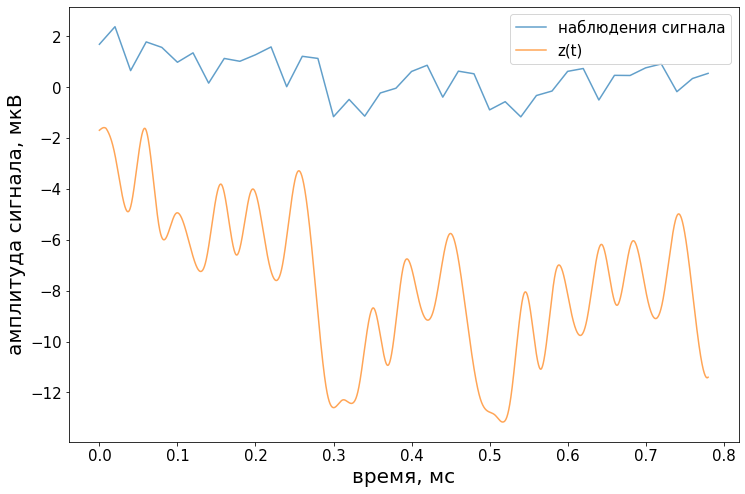
\includegraphics[width=0.8\textwidth]{sections/gorpinich/data.png}
\caption{Time series visualization}
\label{fig:data}
\end{figure}

Fig. \ref{fig:data} plots P300 time series.

\begin{figure}[h!]
\centering
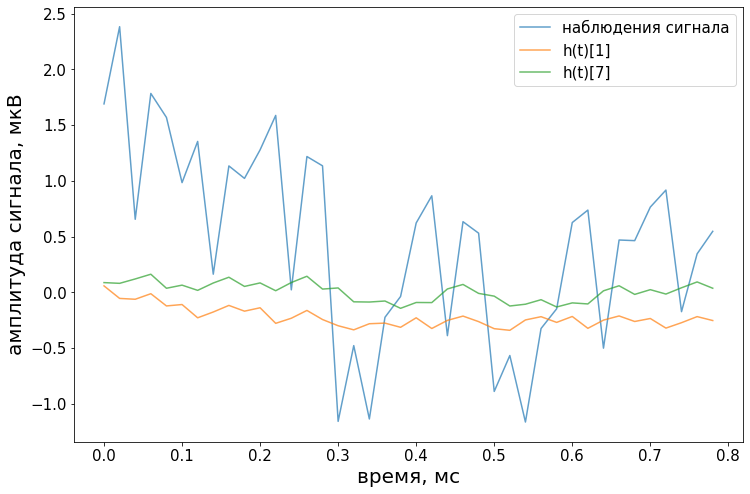
\includegraphics[width=0.8\textwidth]{sections/gorpinich/res.png}
\caption{Result after applying ODE-RNN}
\label{fig:res}
\end{figure}

Fig. \ref{fig:res} plots the result of applying ODE-RNN.

\end{document}